\documentclass[twoside]{book}

% Packages required by doxygen
\usepackage{fixltx2e}
\usepackage{calc}
\usepackage{doxygen}
\usepackage[export]{adjustbox} % also loads graphicx
\usepackage{graphicx}
\usepackage[utf8]{inputenc}
\usepackage{makeidx}
\usepackage{multicol}
\usepackage{multirow}
\PassOptionsToPackage{warn}{textcomp}
\usepackage{textcomp}
\usepackage[nointegrals]{wasysym}
\usepackage[table]{xcolor}

% Font selection
\usepackage[T1]{fontenc}
\usepackage[scaled=.90]{helvet}
\usepackage{courier}
\usepackage{amssymb}
\usepackage{sectsty}
\renewcommand{\familydefault}{\sfdefault}
\allsectionsfont{%
  \fontseries{bc}\selectfont%
  \color{darkgray}%
}
\renewcommand{\DoxyLabelFont}{%
  \fontseries{bc}\selectfont%
  \color{darkgray}%
}
\newcommand{\+}{\discretionary{\mbox{\scriptsize$\hookleftarrow$}}{}{}}

% Page & text layout
\usepackage{geometry}
\geometry{%
  a4paper,%
  top=2.5cm,%
  bottom=2.5cm,%
  left=2.5cm,%
  right=2.5cm%
}
\tolerance=750
\hfuzz=15pt
\hbadness=750
\setlength{\emergencystretch}{15pt}
\setlength{\parindent}{0cm}
\setlength{\parskip}{3ex plus 2ex minus 2ex}
\makeatletter
\renewcommand{\paragraph}{%
  \@startsection{paragraph}{4}{0ex}{-1.0ex}{1.0ex}{%
    \normalfont\normalsize\bfseries\SS@parafont%
  }%
}
\renewcommand{\subparagraph}{%
  \@startsection{subparagraph}{5}{0ex}{-1.0ex}{1.0ex}{%
    \normalfont\normalsize\bfseries\SS@subparafont%
  }%
}
\makeatother

% Headers & footers
\usepackage{fancyhdr}
\pagestyle{fancyplain}
\fancyhead[LE]{\fancyplain{}{\bfseries\thepage}}
\fancyhead[CE]{\fancyplain{}{}}
\fancyhead[RE]{\fancyplain{}{\bfseries\leftmark}}
\fancyhead[LO]{\fancyplain{}{\bfseries\rightmark}}
\fancyhead[CO]{\fancyplain{}{}}
\fancyhead[RO]{\fancyplain{}{\bfseries\thepage}}
\fancyfoot[LE]{\fancyplain{}{}}
\fancyfoot[CE]{\fancyplain{}{}}
\fancyfoot[RE]{\fancyplain{}{\bfseries\scriptsize Generated by Doxygen }}
\fancyfoot[LO]{\fancyplain{}{\bfseries\scriptsize Generated by Doxygen }}
\fancyfoot[CO]{\fancyplain{}{}}
\fancyfoot[RO]{\fancyplain{}{}}
\renewcommand{\footrulewidth}{0.4pt}
\renewcommand{\chaptermark}[1]{%
  \markboth{#1}{}%
}
\renewcommand{\sectionmark}[1]{%
  \markright{\thesection\ #1}%
}

% Indices & bibliography
\usepackage{natbib}
\usepackage[titles]{tocloft}
\setcounter{tocdepth}{3}
\setcounter{secnumdepth}{5}
\makeindex

% Hyperlinks (required, but should be loaded last)
\usepackage{ifpdf}
\ifpdf
  \usepackage[pdftex,pagebackref=true]{hyperref}
\else
  \usepackage[ps2pdf,pagebackref=true]{hyperref}
\fi
\hypersetup{%
  colorlinks=true,%
  linkcolor=blue,%
  citecolor=blue,%
  unicode%
}

% Custom commands
\newcommand{\clearemptydoublepage}{%
  \newpage{\pagestyle{empty}\cleardoublepage}%
}

\usepackage{caption}
\captionsetup{labelsep=space,justification=centering,font={bf},singlelinecheck=off,skip=4pt,position=top}

%===== C O N T E N T S =====

\begin{document}

% Titlepage & ToC
\hypersetup{pageanchor=false,
             bookmarksnumbered=true,
             pdfencoding=unicode
            }
\pagenumbering{roman}
\begin{titlepage}
\vspace*{7cm}
\begin{center}%
{\Large My Project }\\
\vspace*{1cm}
{\large Generated by Doxygen 1.8.11}\\
\end{center}
\end{titlepage}
\clearemptydoublepage
\tableofcontents
\clearemptydoublepage
\pagenumbering{arabic}
\hypersetup{pageanchor=true}

%--- Begin generated contents ---
\chapter{Class Index}
\section{Class List}
Here are the classes, structs, unions and interfaces with brief descriptions\+:\begin{DoxyCompactList}
\item\contentsline{section}{\hyperlink{structEnemy}{Enemy} }{\pageref{structEnemy}}{}
\item\contentsline{section}{\hyperlink{structHero}{Hero} }{\pageref{structHero}}{}
\item\contentsline{section}{\hyperlink{structInput}{Input} }{\pageref{structInput}}{}
\item\contentsline{section}{\hyperlink{structLevel}{Level} }{\pageref{structLevel}}{}
\item\contentsline{section}{\hyperlink{structperso}{perso} }{\pageref{structperso}}{}
\item\contentsline{section}{\hyperlink{structSpell}{Spell} }{\pageref{structSpell}}{}
\end{DoxyCompactList}

\chapter{Class Documentation}
\hypertarget{structEnemy}{}\section{Enemy Struct Reference}
\label{structEnemy}\index{Enemy@{Enemy}}


Collaboration diagram for Enemy\+:
\nopagebreak
\begin{figure}[H]
\begin{center}
\leavevmode
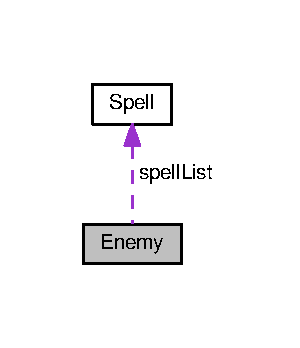
\includegraphics[width=144pt]{structEnemy__coll__graph}
\end{center}
\end{figure}
\subsection*{Public Attributes}
\begin{DoxyCompactItemize}
\item 
int {\bfseries id}\hypertarget{structEnemy_a70490642cc6e18ad3d0284dfa1930af3}{}\label{structEnemy_a70490642cc6e18ad3d0284dfa1930af3}

\item 
char {\bfseries name} \mbox{[}50\mbox{]}\hypertarget{structEnemy_a6c62136940d4dd9dd0c2a4cd7f8b1281}{}\label{structEnemy_a6c62136940d4dd9dd0c2a4cd7f8b1281}

\item 
int {\bfseries max\+HP}\hypertarget{structEnemy_a990ecf4cbfdae850b51e6fb2b367ad8e}{}\label{structEnemy_a990ecf4cbfdae850b51e6fb2b367ad8e}

\item 
int {\bfseries max\+AP}\hypertarget{structEnemy_aeae465e0f4dc57942fefa05801b8d35e}{}\label{structEnemy_aeae465e0f4dc57942fefa05801b8d35e}

\item 
int {\bfseries current\+HP}\hypertarget{structEnemy_a2891f607bd7c05774ab7efaf155c1842}{}\label{structEnemy_a2891f607bd7c05774ab7efaf155c1842}

\item 
int {\bfseries current\+AP}\hypertarget{structEnemy_a5abcfd0d6c94e944f4d360eaa55697ef}{}\label{structEnemy_a5abcfd0d6c94e944f4d360eaa55697ef}

\item 
int {\bfseries spawn\+PointX}\hypertarget{structEnemy_a74809a13404cfdb35d7d565f3f11721a}{}\label{structEnemy_a74809a13404cfdb35d7d565f3f11721a}

\item 
int {\bfseries spawn\+PointY}\hypertarget{structEnemy_a99846a4490691509b7dff6ec1883d619}{}\label{structEnemy_a99846a4490691509b7dff6ec1883d619}

\item 
int {\bfseries range}\hypertarget{structEnemy_a78afb6ee76a1d0e570e17b75f81736ed}{}\label{structEnemy_a78afb6ee76a1d0e570e17b75f81736ed}

\item 
int {\bfseries leftcounter}\hypertarget{structEnemy_af0807029db68e4f2573487e20786c3d4}{}\label{structEnemy_af0807029db68e4f2573487e20786c3d4}

\item 
int {\bfseries rightcounter}\hypertarget{structEnemy_a430ccb5b75909614f2f485f43ed44cc9}{}\label{structEnemy_a430ccb5b75909614f2f485f43ed44cc9}

\item 
int {\bfseries upcounter}\hypertarget{structEnemy_acb602ccb569b15f5eba388f46fa81495}{}\label{structEnemy_acb602ccb569b15f5eba388f46fa81495}

\item 
int {\bfseries downcounter}\hypertarget{structEnemy_af9c30e625005a209649cf8e3e392b5b6}{}\label{structEnemy_af9c30e625005a209649cf8e3e392b5b6}

\item 
direction {\bfseries d}\hypertarget{structEnemy_a2bd91391c42800869f146cee2590d529}{}\label{structEnemy_a2bd91391c42800869f146cee2590d529}

\item 
S\+D\+L\+\_\+\+Rect {\bfseries pos}\hypertarget{structEnemy_ab5abf403ad6178b1046732d9df2db0c1}{}\label{structEnemy_ab5abf403ad6178b1046732d9df2db0c1}

\item 
S\+D\+L\+\_\+\+Surface $\ast$ {\bfseries up\+Image} \mbox{[}4\mbox{]}\hypertarget{structEnemy_aab554cf0e1bc2eff76a4c4133fc8324e}{}\label{structEnemy_aab554cf0e1bc2eff76a4c4133fc8324e}

\item 
S\+D\+L\+\_\+\+Surface $\ast$ {\bfseries down\+Image} \mbox{[}4\mbox{]}\hypertarget{structEnemy_acaffe5b866d91cd19887eb365b948b2a}{}\label{structEnemy_acaffe5b866d91cd19887eb365b948b2a}

\item 
S\+D\+L\+\_\+\+Surface $\ast$ {\bfseries right\+Image} \mbox{[}4\mbox{]}\hypertarget{structEnemy_a79ff16d49480136bdaeebe8089c47e97}{}\label{structEnemy_a79ff16d49480136bdaeebe8089c47e97}

\item 
S\+D\+L\+\_\+\+Surface $\ast$ {\bfseries left\+Image} \mbox{[}4\mbox{]}\hypertarget{structEnemy_aba228b85b8e14c26edbfbfe0f7b1e301}{}\label{structEnemy_aba228b85b8e14c26edbfbfe0f7b1e301}

\item 
S\+D\+L\+\_\+\+Surface $\ast$ {\bfseries battle\+Image}\hypertarget{structEnemy_ad389759926772fb4442b5ce64f32b9dd}{}\label{structEnemy_ad389759926772fb4442b5ce64f32b9dd}

\item 
\hyperlink{structSpell}{Spell} {\bfseries spell\+List} \mbox{[}4\mbox{]}\hypertarget{structEnemy_a63ecb64ded9f4198bf2771158c8571b2}{}\label{structEnemy_a63ecb64ded9f4198bf2771158c8571b2}

\end{DoxyCompactItemize}


The documentation for this struct was generated from the following file\+:\begin{DoxyCompactItemize}
\item 
Header.\+h\end{DoxyCompactItemize}

\hypertarget{structHero}{}\section{Hero Struct Reference}
\label{structHero}\index{Hero@{Hero}}


Collaboration diagram for Hero\+:
\nopagebreak
\begin{figure}[H]
\begin{center}
\leavevmode
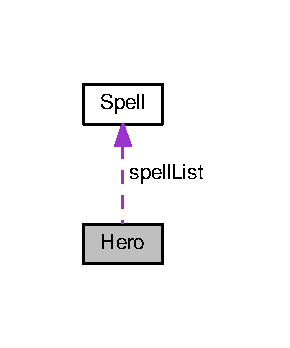
\includegraphics[width=139pt]{structHero__coll__graph}
\end{center}
\end{figure}
\subsection*{Public Attributes}
\begin{DoxyCompactItemize}
\item 
int {\bfseries id}\hypertarget{structHero_a8e0b7a82c8ebbbb0a94cdb00d8ba52ee}{}\label{structHero_a8e0b7a82c8ebbbb0a94cdb00d8ba52ee}

\item 
char {\bfseries name} \mbox{[}50\mbox{]}\hypertarget{structHero_a947928d6a97732c9eb622c758dc00aa9}{}\label{structHero_a947928d6a97732c9eb622c758dc00aa9}

\item 
int {\bfseries max\+HP}\hypertarget{structHero_a28b2bffc01d17d1df0904169acfabac7}{}\label{structHero_a28b2bffc01d17d1df0904169acfabac7}

\item 
int {\bfseries max\+AP}\hypertarget{structHero_a42f1b98ece3101ffe87b49b4d347e1d5}{}\label{structHero_a42f1b98ece3101ffe87b49b4d347e1d5}

\item 
int {\bfseries current\+HP}\hypertarget{structHero_a7c2adb58fafd935f013847a9383ab755}{}\label{structHero_a7c2adb58fafd935f013847a9383ab755}

\item 
int {\bfseries current\+AP}\hypertarget{structHero_a9970c3ae5e2bbf99060dfd062f3739fc}{}\label{structHero_a9970c3ae5e2bbf99060dfd062f3739fc}

\item 
S\+D\+L\+\_\+\+Surface $\ast$ {\bfseries up\+Image} \mbox{[}4\mbox{]}\hypertarget{structHero_a37717fa64696425f7af82f37cb6dca62}{}\label{structHero_a37717fa64696425f7af82f37cb6dca62}

\item 
S\+D\+L\+\_\+\+Surface $\ast$ {\bfseries down\+Image} \mbox{[}4\mbox{]}\hypertarget{structHero_a0082a2d40be4239acb9fd602bcc85585}{}\label{structHero_a0082a2d40be4239acb9fd602bcc85585}

\item 
S\+D\+L\+\_\+\+Surface $\ast$ {\bfseries right\+Image} \mbox{[}4\mbox{]}\hypertarget{structHero_a861267c33724070c1f9d50c9e4f5d94e}{}\label{structHero_a861267c33724070c1f9d50c9e4f5d94e}

\item 
S\+D\+L\+\_\+\+Surface $\ast$ {\bfseries left\+Image} \mbox{[}4\mbox{]}\hypertarget{structHero_a15b94881c772aad2443f64104bb799ce}{}\label{structHero_a15b94881c772aad2443f64104bb799ce}

\item 
S\+D\+L\+\_\+\+Surface $\ast$ {\bfseries battle\+Image}\hypertarget{structHero_af12606b16996c2118f0deb3808926d64}{}\label{structHero_af12606b16996c2118f0deb3808926d64}

\item 
\hyperlink{structSpell}{Spell} {\bfseries spell\+List} \mbox{[}4\mbox{]}\hypertarget{structHero_ae17ce17d4329b5a22de4a1a929efe76d}{}\label{structHero_ae17ce17d4329b5a22de4a1a929efe76d}

\end{DoxyCompactItemize}


The documentation for this struct was generated from the following file\+:\begin{DoxyCompactItemize}
\item 
Header.\+h\end{DoxyCompactItemize}

\hypertarget{structInput}{}\section{Input Struct Reference}
\label{structInput}\index{Input@{Input}}
\subsection*{Public Attributes}
\begin{DoxyCompactItemize}
\item 
char {\bfseries key} \mbox{[}S\+D\+L\+K\+\_\+\+L\+A\+ST\mbox{]}\hypertarget{structInput_a211bceabbcc2ccdd710502d596692ab5}{}\label{structInput_a211bceabbcc2ccdd710502d596692ab5}

\end{DoxyCompactItemize}


The documentation for this struct was generated from the following file\+:\begin{DoxyCompactItemize}
\item 
perso.\+h\end{DoxyCompactItemize}

\hypertarget{structLevel}{}\section{Level Struct Reference}
\label{structLevel}\index{Level@{Level}}
\subsection*{Public Attributes}
\begin{DoxyCompactItemize}
\item 
int {\bfseries id}\hypertarget{structLevel_acd7d99360a99ebbe89a9410c1741ae4b}{}\label{structLevel_acd7d99360a99ebbe89a9410c1741ae4b}

\item 
int {\bfseries enemy\+Count}\hypertarget{structLevel_a2ba7dc6170abe47fefb58c0d9693ce83}{}\label{structLevel_a2ba7dc6170abe47fefb58c0d9693ce83}

\item 
char {\bfseries enemy\+File} \mbox{[}50\mbox{]}\hypertarget{structLevel_ad9fda26f018b4a77811e5414cbbde94b}{}\label{structLevel_ad9fda26f018b4a77811e5414cbbde94b}

\item 
S\+D\+L\+\_\+\+Rect {\bfseries start\+Pos}\hypertarget{structLevel_a23eb66e4415bfce1aba099aae8f9ac3d}{}\label{structLevel_a23eb66e4415bfce1aba099aae8f9ac3d}

\item 
S\+D\+L\+\_\+\+Rect {\bfseries end\+Pos}\hypertarget{structLevel_a81d6d6465e52d6b57c598dd640f509a6}{}\label{structLevel_a81d6d6465e52d6b57c598dd640f509a6}

\item 
char {\bfseries map\+File} \mbox{[}50\mbox{]}\hypertarget{structLevel_a68be9f0ecb50b6384393d338ec532124}{}\label{structLevel_a68be9f0ecb50b6384393d338ec532124}

\item 
char {\bfseries map\+Collision} \mbox{[}50\mbox{]}\hypertarget{structLevel_abd053e36f179534d1a3c70fd30060673}{}\label{structLevel_abd053e36f179534d1a3c70fd30060673}

\end{DoxyCompactItemize}


The documentation for this struct was generated from the following file\+:\begin{DoxyCompactItemize}
\item 
Header.\+h\end{DoxyCompactItemize}

\hypertarget{structperso}{}\section{perso Struct Reference}
\label{structperso}\index{perso@{perso}}
\subsection*{Public Attributes}
\begin{DoxyCompactItemize}
\item 
S\+D\+L\+\_\+\+Surface $\ast$ {\bfseries image}\hypertarget{structperso_a3bb43b8e820b3ba348b6c96458b39231}{}\label{structperso_a3bb43b8e820b3ba348b6c96458b39231}

\item 
S\+D\+L\+\_\+\+Rect {\bfseries frame}\hypertarget{structperso_a1131a2be46ede188e4a1b1deaa571ac3}{}\label{structperso_a1131a2be46ede188e4a1b1deaa571ac3}

\item 
S\+D\+L\+\_\+\+Rect {\bfseries position}\hypertarget{structperso_a74aed265eb926987cf218b19d163c746}{}\label{structperso_a74aed265eb926987cf218b19d163c746}

\item 
int {\bfseries vi}\hypertarget{structperso_a115e2208c9a6a45d36b951d04fb2fb1f}{}\label{structperso_a115e2208c9a6a45d36b951d04fb2fb1f}

\item 
int {\bfseries coins}\hypertarget{structperso_a06566a4a0b1f89c646a9aafa6cee700d}{}\label{structperso_a06566a4a0b1f89c646a9aafa6cee700d}

\item 
int {\bfseries HP}\hypertarget{structperso_ae47b9a8af2af325d2442024a7135d4db}{}\label{structperso_ae47b9a8af2af325d2442024a7135d4db}

\end{DoxyCompactItemize}


The documentation for this struct was generated from the following file\+:\begin{DoxyCompactItemize}
\item 
perso.\+h\end{DoxyCompactItemize}

\hypertarget{structSpell}{}\section{Spell Struct Reference}
\label{structSpell}\index{Spell@{Spell}}
\subsection*{Public Attributes}
\begin{DoxyCompactItemize}
\item 
int {\bfseries id}\hypertarget{structSpell_a1326be69cf181af817be2848680d12e7}{}\label{structSpell_a1326be69cf181af817be2848680d12e7}

\item 
char {\bfseries name} \mbox{[}50\mbox{]}\hypertarget{structSpell_a02a908f6bb055b1220ff2c2526286a78}{}\label{structSpell_a02a908f6bb055b1220ff2c2526286a78}

\item 
int {\bfseries damage}\hypertarget{structSpell_a375d0e94137a43f4ffd761dfe6ab0c3f}{}\label{structSpell_a375d0e94137a43f4ffd761dfe6ab0c3f}

\item 
int {\bfseries heal}\hypertarget{structSpell_a759e8ee282eb0c06d6bdade83ec4c0fa}{}\label{structSpell_a759e8ee282eb0c06d6bdade83ec4c0fa}

\item 
int {\bfseries AP}\hypertarget{structSpell_aeb47cca9bf674355e767e6b3b20674f8}{}\label{structSpell_aeb47cca9bf674355e767e6b3b20674f8}

\item 
int {\bfseries critchance}\hypertarget{structSpell_a2febe0d6e9c46148d392bb357d52ee7b}{}\label{structSpell_a2febe0d6e9c46148d392bb357d52ee7b}

\end{DoxyCompactItemize}


The documentation for this struct was generated from the following file\+:\begin{DoxyCompactItemize}
\item 
Header.\+h\end{DoxyCompactItemize}

%--- End generated contents ---

% Index
\backmatter
\newpage
\phantomsection
\clearemptydoublepage
\addcontentsline{toc}{chapter}{Index}
\printindex

\end{document}
